%!TEX root = pixel-wise-street-segmentation.tex

\section{Experimental Results}\label{sec:evaluation}

In this section we discuss the experimental results of the models
presented in \cref{sec:model}. First, we evaluate the two different
models. Second, we compare our best one to the work of
Mohan~\cite{Tarel2009} (which is ranked on place~1 at KITTI road
segmentation~\cite{Tarel2009}). The KITTI Road Estimation data set is the basis
of our experiments (see \cref{sec:datasets}). \\
%!TEX root = pixel-wise-street-segmentation.tex

\subsection{Data Sets}\label{sec:datasets}
The KITTI Road Estimation data set~\cite{Fritsch2013} was used for training of
the models and for obtaining the experimental results reported in
\cref{sec:evaluation}.

The left color image base kit contains a training and a test set. All photos
are in an urban environment. The training set has 95~photos with land markings
(um), 96~photos with multiple lane markings (umm) and 98~photos where the
street has no lane markings (uu). The test set has 96~um~photos, 94~umm~photos
and 100~uu~photos.

The width of all photos is in $\Set{1226, 1238, 1241, 1242}$, the height is in
$\Set{370, 374, 375, 376}$.

The data photos are given as 8-bit color RGB PNG files. The labels (ground
truth) are given as images of the same size as the data image, but with only
three colors: red (\verb+#ff0000+), magenta (\verb+#ff00ff+) for street and
black (\verb+#000000+) for other streets than the one the car is on.

\subsection{Metrics / Experiments}
To be able to evaluate different approaches we used only the
training data of the KITTI data set, as the ground truth for the test data is
not publicly available. We splitted the training data beforehand 20 to 80
(test/training) in order to be able to measure our performance. Our best model
was submitted for the official KITTI evaluation
(\href{http://www.cvlibs.net/datasets/kitti/eval_road.php}{www.cvlibs.net/datasets/kitti/eval\_road.php})


Our goal was to achieve an adequate classification performance while staying
within a time frame of \textbf{\SI{20}{\milli\second}} as maximal
classification time per image. Resulting in a usable real time application of
our approach. As a real time application would be the use case for street
classification in autonomous cars anyway.\\

We used a computer with these specifications for the experiments (GPU was used
for training and testing):
\begin{itemize}
    \item Intel(R) Core(TM) i7-4790K CPU @ \SI{4.00}{\giga\hertz}
    \item System memory \SI{16}{\gibi\byte}
    \item GeForce GTX 980 \SI{4}{\gibi\byte} RAM
\end{itemize}

\begin{table}[]
    \begin{center}
        \begin{tabular}{c|cccccc}
            \toprule
            \textbf{Model} & {\bf $\mathbf{F_1}$} & \textbf{TN} & \textbf{FP} & \textbf{FN} & \textbf{TP} & \textbf{ACC} \\
            \midrule
            \textbf{Reg., $s=10$} & \SI{88.0}{\percent} & \SI{97.8}{\percent} & \SI{2.2}{\percent}& \SI{19.7}{\percent}& \SI{80.2}{\percent}& \SI{94.7}{\percent}\\
            \textbf{Reg., $s=37$} & \SI{89.0}{\percent}& \SI{97.3}{\percent}& \SI{2.6}{\percent}& \SI{17.6}{\percent}& \SI{82.3}{\percent} &  \textcolor{red}{\SI{94.8}{\percent}}\\
            \textbf{Reg., $s=51$} & \textcolor{red}{\SI{89.5}{\percent}} &\SI{96.9}{\percent} & \SI{3.1}{\percent} & \SI{16.5}{\percent}& \textcolor{red}{\SI{83.5}{\percent}} & \SI{94.6}{\percent}\\
            \midrule
            \textbf{Cla., $s=10$} & \SI{85.4}{\percent} & \SI{98.1}{\percent}& \SI{1.9}{\percent}&\SI{24.1}{\percent} & \SI{75.8}{\percent} & \SI{94.2}{\percent}\\
            \textbf{Cla., $s=37$} & \SI{86.2}{\percent}& \SI{95.9}{\percent} & \SI{4.1}{\percent} & \SI{21.2}{\percent} & \SI{78.7}{\percent} & \SI{92.9}{\percent}\\
            \textbf{Cla., $s=51$} & \SI{70.1}{\percent} & \textcolor{red}{\SI{98.2}{\percent}} & \SI{1.8}{\percent} & \SI{45.1}{\percent} & \SI{54.9}{\percent} & \SI{90.6}{\percent}\\
            \bottomrule
        \end{tabular}
        \caption{Results of classification (cla.) and regression (reg.) models
                 with different strides $s$ on our own test set (58~images,
                 $ ~6.7 \cdot 10^6$ pixels). The table entries highlighted in
                 red are the best results of their column.}
        \label{tab:ownapproach}
    \end{center}
\end{table}

\Cref{tab:ownapproach} shows the result of our evaluation and regression
approach using the models and parameters as described in \cref{sec:model}. The
used score is the $F_1$-measure \cref{eq:fMeasure} which is also used in the
official KITTI evaluation. The table also shows the values of true positive
(TP), true negative (TN), false positive (FP), false negative (FN) and accuracy
(ACC) \cref{eq:accuracy}. It shows clearly that the regression model has an
overall better $F_1$-measure and accuracy score than the classification model.
Surprisingly, a smaller stride does not automatically lead to a better
performance. The classification model shows with a stride of the size 37 the
best result, while in the regression based approach a stride of 51 achieves the
best performance. Unfortunately the ram of the graphic card limited our
possibility to use larger strides and patch sizes. This could have been a
promising possibility to train and evaluate on a full image size and still keep
our time constraint and even enhance our performance.\\

\begin{equation} \label{eq:fMeasure}
F_1-\text{measure} = \frac{2 \cdot TP}{2TP +FP +FN}
\end{equation}
\begin{equation} \label{eq:accuracy}
\text{accuracy} = \frac{TP + TN}{TP + FP + TN + FN}
\end{equation}

\begin{table}[]
    \begin{center}
        \begin{tabular}{c|ccc}
            \toprule
            \textbf{network type/stride} & \textbf{10} & \textbf{37} & \textbf{51} \\
            \midrule
            \textbf{regression}     & 1.99 & 0.29 & 0.18 \\
            \textbf{classification} & 1.83 & 0.2  & 0.11\\
            \bottomrule
        \end{tabular}
        \caption{Runtime per image ($621 \times 188$ pixel) in seconds.}
        \label{tab:runtime}
    \end{center}
\end{table}

\begin{figure*}[]
    \begin{subfigure}[t]{\columnwidth}
        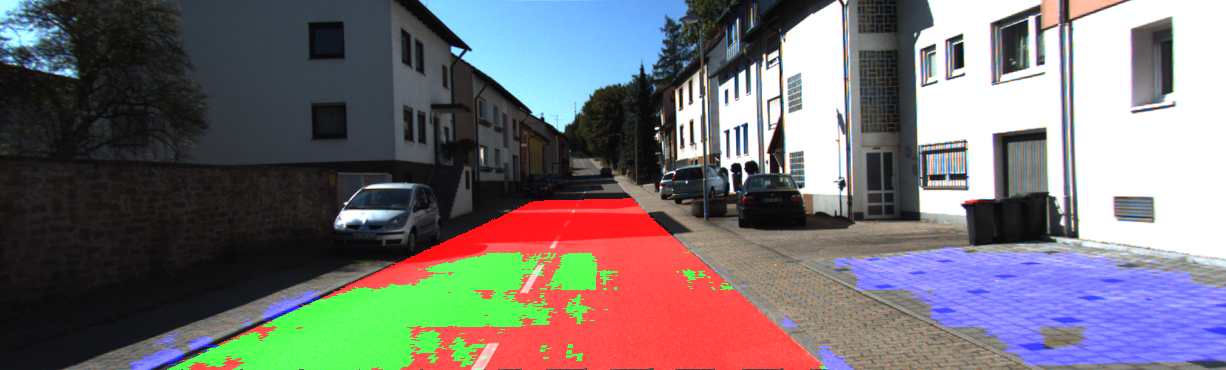
\includegraphics[width=\columnwidth]{figures/kitti_eval/Persp_um_road_000077.png}
        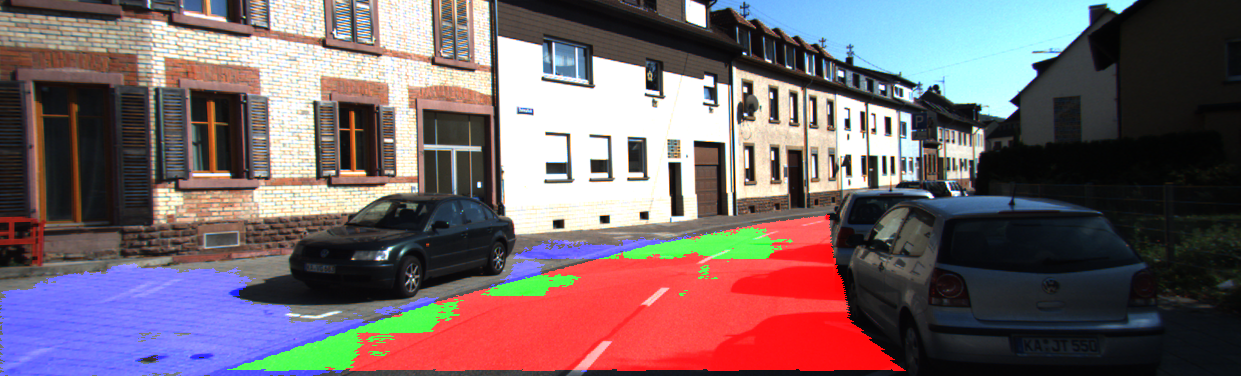
\includegraphics[width=\columnwidth]{figures/kitti_eval/Persp_um_road_000095.png}
        \caption{Shows KITTI test data on which our neural net performed badly. Here, red denotes false negatives, blue areas correspond to false positives and green represents true positives.}
        \label{fig:sfig1}
    \end{subfigure}
    \begin{subfigure}[t]{\columnwidth}
        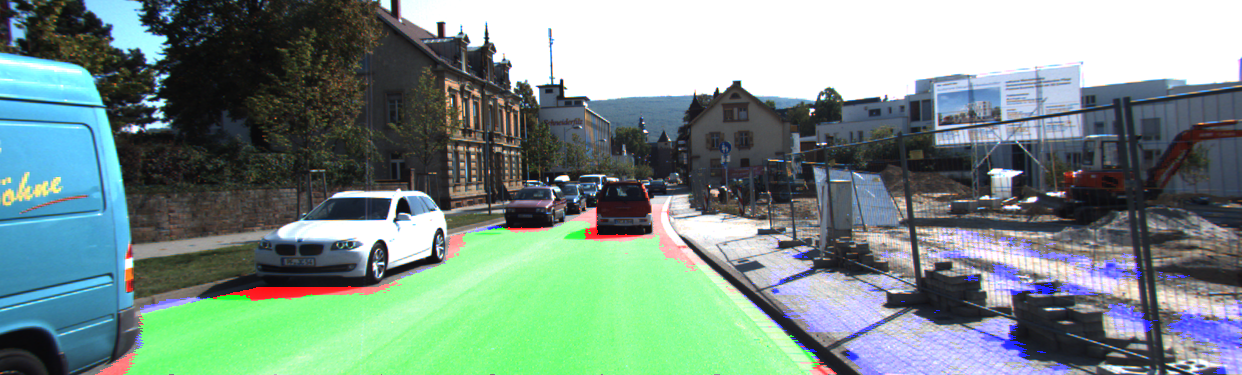
\includegraphics[width=\columnwidth]{figures/kitti_eval/Persp_uu_road_000027.png}
        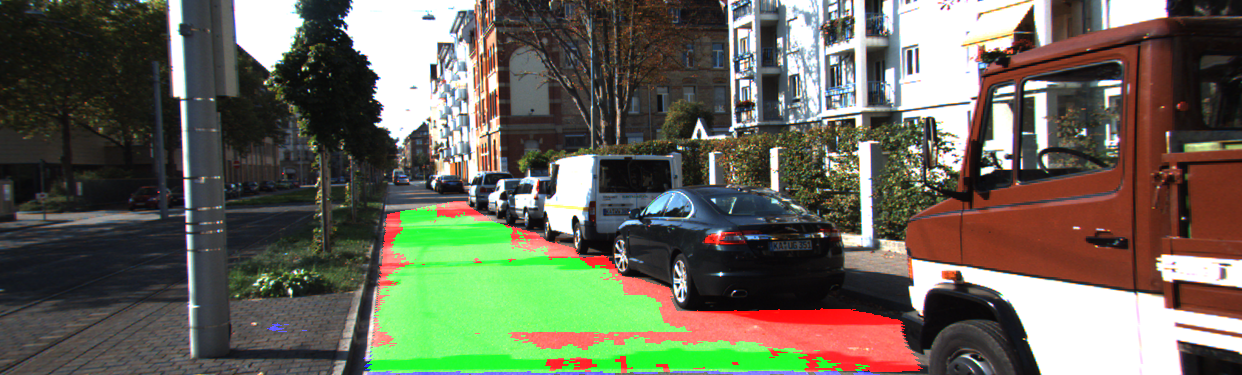
\includegraphics[width=\columnwidth]{figures/kitti_eval/Persp_uu_road_000082.png}
        \caption{Shows KITTI test data on which our neural net performed well.}
        \label{fig:sfig2}
    \end{subfigure}
\end{figure*}

\begin{table*}[]
    \begin{center}
    \begin{tabular}{c|cccccc}
        \toprule
        {\bf Benchmark} & {\bf $\mathbf{F_1}$} & {\bf AP} & {\bf PRE} & {\bf REC} & {\bf FPR} & {\bf FNR}\\
        \midrule
        UM    & \SI{67.91}{\percent} & \SI{61.63}{\percent} & \SI{86.90}{\percent} & \SI{55.74}{\percent} & \SI{3.83}{\percent} & \SI{44.26}{\percent}\\
        UMM   & \SI{79.67}{\percent} & \SI{78.41}{\percent} & \SI{93.29}{\percent} & \SI{69.51}{\percent} & \SI{5.50}{\percent} & \SI{30.49}{\percent}\\
        UU    & \SI{56.48}{\percent} & \SI{51.89}{\percent} & \SI{84.67}{\percent} & \SI{42.37}{\percent} & \SI{2.50}{\percent} & \SI{57.63}{\percent}\\
        URBAN & \SI{71.10}{\percent} & \SI{65.14}{\percent} & \SI{89.83}{\percent} & \SI{58.84}{\percent} & \SI{3.67}{\percent} & \SI{41.16}{\percent}\\
        \bottomrule
        \end{tabular}
    \end{center}
    \caption{Results of the official KITTI evaluation. (AP = Average Precision, PRE = Precision, REC = Recall, FPR = False Positive Rate, FNR = False Negative Rate)}
    \label{tab:kitti}
\end{table*}

To evaluate if we could meet our predefined time constraint (classification of
one image in under \SI{20}{\milli\second}) we conducted a run time evaluation
which is shown in \Cref{tab:runtime}. As expected, the runtime increases with a
smaller stride size. The classification model shows an overall faster run time
performance as the regression. Finally, we managed to achieve a run time under
\SI{20}{\milli\second} by using a stride of $s=51$ in both approaches.

As the regression approach had the best performance and also met our time
constraint, we used it to evaluate the KITTI test set and submitted the results
after a transformation into birds eye view (KITTI
specifications).\Cref{tab:kitti} shows the results which are split into the
different road types (UM, UMM, UU, URBAN).
Unfortunately, our regression model performs much worse on the official test
set than on our own test set. Here the $F_1$-measure score ranges between
\SI{56.4}{\percent} and \SI{79.7}{\percent} while Mohan ~\cite{Tarel2009}
achieves on all road categories a $F_1$-measure score of about
\SI{90.0}{\percent}. The reason for this huge difference to might be: \\

\begin{enumerate}
    \item Overfitting of the neural network on our own test data
    \item Specialization of our two models on images with half the original
          size (the KITTI evaluation is done on full size images)
    \item Visible in the two images of \cref{fig:sfig1} is an example of very
          bad performance on a part of the test image data. Basically more
          non-street is classified as street and most of the street is not
          recognized as one at all. This could be due to the fact of shadows
          in some parts of the street and a bit different color of this
          particular street than most of the street our neural network has
          learned in the training.
\end{enumerate}
To improve the latter it would be essential to use training data of a lot more
different street types and lighting conditions.\\
Finally \cref{fig:sfig2} gives some positives example where our neural network
did well. Hardly no false positives and the street around the cars is nicely
segmented.


%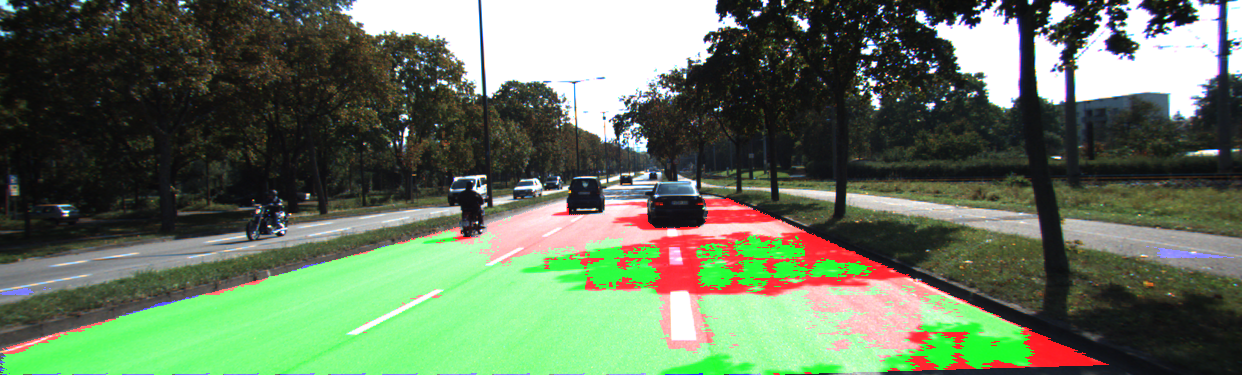
\includegraphics[scale=0.2]{figures/kitti_eval/Persp_umm_road_000025.png}
%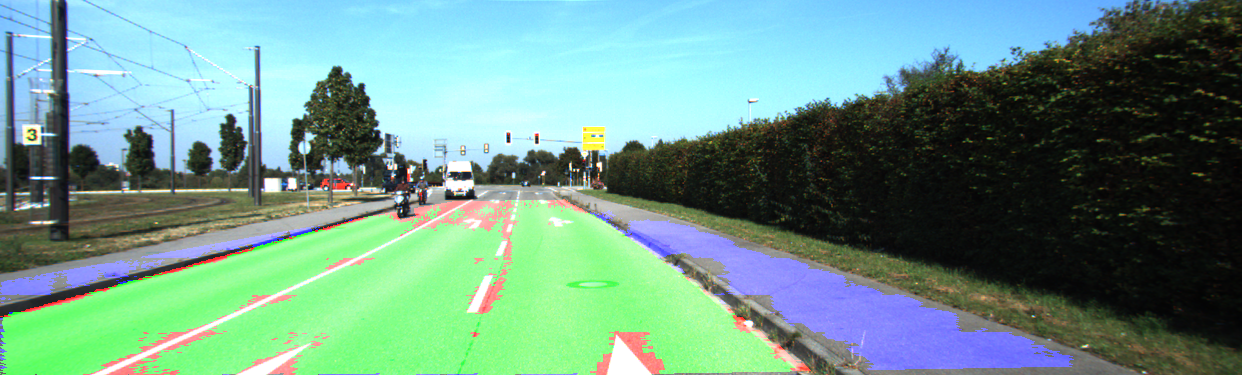
\includegraphics[scale=0.2]{figures/kitti_eval/Persp_umm_road_000040.png}
%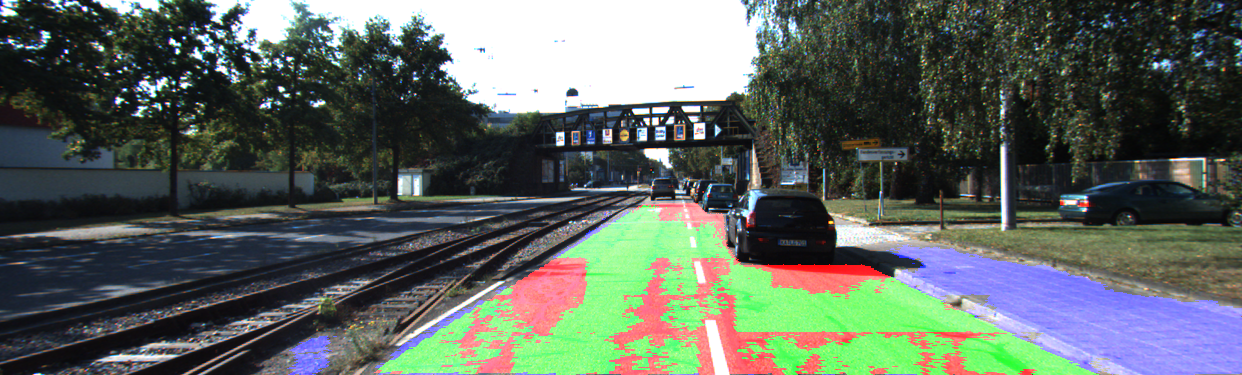
\includegraphics[scale=0.2]{figures/kitti_eval/Persp_umm_road_000066.png}
%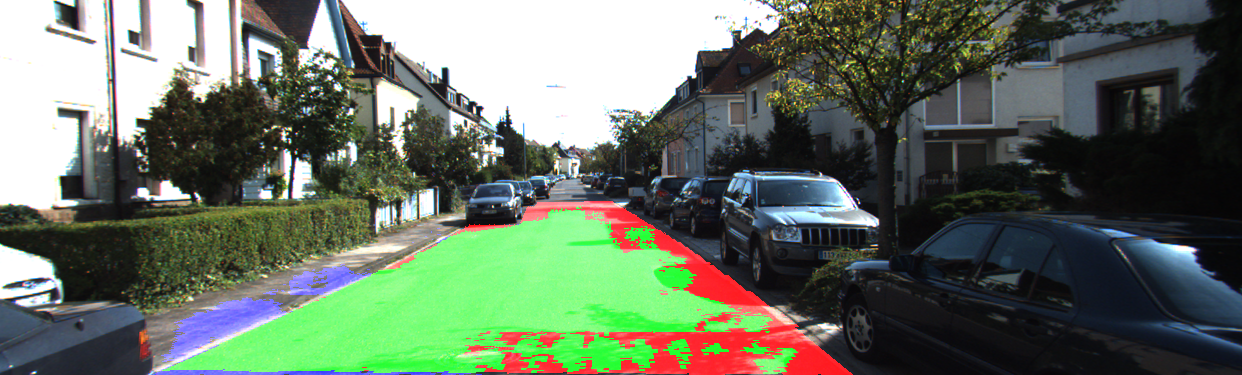
\includegraphics[scale=0.2]{figures/kitti_eval/Persp_uu_road_000020.png}
